\chapter{Frama-C}
\label{sec:framaC}

\section{Presentation}
\begin{description}
\item[\textcolor{green}{Author}] Virgile Prevosto - CEA LIST
\item[\textcolor{blue}{Assessor 1}] First assessor of the approaches \todo{Name - Company}
\item[\textcolor{magenta}{Assessor 2}] Second assessor of the approaches \todo{Name - Company}
\end{description}

\begin{description}
\item[Name] Frama-C
\item[Web site] \url{http://frama-c.com}
\item[Licence] LGPL 2.1
\end{description}

\paragraph{Abstract}
Frama-C is a framework dedicated to the analysis of C programs. It comes
with a formal specification language, ACSL, that allows to describe the
contracts that each function is supposed to fulfill It features a
number of plug-ins that perform various verification tasks. In particular,
Value analysis is an abstract interpretation-based plugin that can verify the
absence of run-time error for any execution of the program, and WP is an 
Hoare-logic based plug-in that can modularly check that an implementation
is conforming to its ACSL specification with the help of automated theorem
provers. Frama-C is also meant to be extensible, and it is easy to tailor
the generic plugins toward specific VnV tasks.

\paragraph{Publications}
\begin{itemize}
\item Pascal Cuoq, Florent Kirchner, Nikolai Kosmatov, Virgile Prevosto,
  Julien Signoles and Boris Yakobowski. Frama-C: a Software Analysis
  Perspective. Proceedings of SEFM 2012.
\item Loïc Correnson and Julien Signoles. Combining Analysises for
  C Program Verification. Proceedings of FMICS 2012
\item Jochen Burghardt, Jens Gerlach, Kerstin Hartig, Hans Pohl and Juan Soto.
  ACSL by Example, a fairly complete tour of ACSL features through
  various functions inspired from C++ STL.
\item Patrick Baudin, Loïc Correnson and Zaynah Dargaye, WP plugin manual.
\url{http://frama-c.com/download/wp-manual-Fluorine-20130601.pdf}
\item Pascal Cuoq, Boris Yakobowski and Virgile Prevosto.
  Frama-C's value analysis plugin manual. 
  \url{http://frama-c.com/download/frama-c-value-analysis.pdf}
\end{itemize}


\section{Common criteria on secondary means and tools}
\label{sec:frama-c-common}
This section discusses the common criteria of the means and tools according to the project requirements on tools and the results of T7.1.

\subsection{Project and WP2 requirements}

The objectives of this list of criteria is to check if the proposed means and tools meet the main criteria of the project: open-source approaches, usability, modularity, coverage of the objectives,...

According WP2 requirements, give a note for characteristics of the use of the tool (from 0 to 3) :

\begin{tabular}{|l | c | c | c | c|}
\hline
& \textcolor{green}{Author} & \textcolor{blue}{Assessor 1} & \textcolor{magenta}{Assessor 2} & Total \\
\hline 
Open Source (D2.6-02-074) & 3 & & &  \\
\hline 
Portability to operating systems (D2.6-02-075) & 2 & & &  \\
\hline
Cooperation of tools (D2.6-02-076) & 1 & & &  \\
\hline
Robustness (D2.6-02-078) & 2 & & & \\
\hline
Modularity (D2.6-02-078.1) & 2 & & & \\
\hline
Documentation management (D2.6-02-078.02) & 0 & & & \\
\hline
Distributed software development (D2.6-02-078.03)  & 0 & & & \\
\hline
Simultaneous multi-users (D2.6-02-078.04)   & * & & & \\
\hline
Issue tracking (D2.6-02-078.05) & 0 & & & \\
\hline
Differences between models (D2.6-02-078.06) & 0 & & & \\
\hline
Version management (D2.6-02-078.07) & 0 & & & \\
\hline
Concurrent version development (D2.6-02-078.08) & 0 & & & \\
\hline
Model-based version control (D2.6-02-078.09) & 0 & & & \\
\hline
Role traceability (D2.6-02-078.10) & 0 & & & \\
\hline
Safety version traceability (D2.6-02-078.11) & 0 & & & \\
\hline
Model traceability (D2.6-02-079) & 0 & & & \\
\hline
Tool chain integration & 1 & & & \\
\hline
Scalability & 2 & & & \\
\hline
User Friendliness & 1 & & & \\
\hline
\end{tabular}

\begin{author_comment}
\begin{itemize}
\item Frama-C works on Linux, Windows and MacOS X, 
but must be compiled from source, which is not always very easy on Windows.
\item Cooperation can mainly be envisaged
in the form of generation of ACSL specification from SysML/Scade, but there is
no existing plug-in for that.
\item An Eclipse plug-in is available 
(FCDT: \url{http://gforge.enseeiht.fr/projects/fcdt/}) for launching some
analyses from Eclipse.
\end{itemize}
\end{author_comment}


\subsection{Qualification}

This section discusses how the tool can be classified according EN50128 requirements (D2.6-02-085). Some qualification shall be mandatory  if the tool is involved to design a SIL4 software.


\begin{tabular}{|l | c | c | c | c|}
\hline
& \textcolor{green}{Author} & \textcolor{blue}{Assessor 1} & \textcolor{magenta}{Assessor 2} & Total \\
\hline 
Tool manual (D.2.6-01-42.02) & 2 & & &  \\
\hline
Proof of correctness (D.2.6-01-42.03)   & 2 & & & \\
\hline
Existing industrial  usage  & 1 & & & \\
\hline
Model verification & 0 & & & \\
\hline
Test generation & * & & & \\
\hline
Simulation, execution, debugging & 2 & & & \\
\hline
Formal proof & 3 & & & \\
\hline
\end{tabular}

\begin{author_comment}
There exists a test-case generator plugin, but it is not distributed
under an Open-Source licence. Value Analysis plugin can be tweaked into an
interpreter/simulator if needed
\end{author_comment}

Which level of tool qualification has been reached or will be reached within the next year ?

Score :
\begin{description}
\item[3] already qualified for this level
\item[2] qualification possible to this level, but some elements shall be provided
\item[0] qualification not recommended for this level
\end{description}


\begin{tabular}{|l | c | c | c | c|}
\hline
& \textcolor{green}{Author} & \textcolor{blue}{Assessor 1} & \textcolor{magenta}{Assessor 2} & Total \\
\hline 
class T1 & 1 & & &  \\
\hline
class T2   & 1 & & & \\
\hline
class T3  & 1 & & & \\
\hline
\end{tabular}

\begin{author_comment}
There has been some reflection on the qualification of Frama-C with respect to
DO-178 verification activities, but no formal process has taken place yet.
\end{author_comment}

\paragraph{Other elements for tool certification}


\subsection{Complementarity with primary toolchain}

The objectives of this list of criteria is to check if the proposed means and tools can be easily integrated to the primary toolchain.

\subsubsection{Language}
\label{sec:Frama-C:language}

According to the decisions and the propositions of T7.1, how the mean and approach can be adapted to or can complete the chosen language and methods:

\begin{tabular}{|l | c | c | c | c|}
\hline
& \textcolor{green}{Author} & \textcolor{blue}{Assessor 1} & \textcolor{magenta}{Assessor 2} & Total \\
\hline 
SysML  & 1 & & & \\
\hline
Scade method & 2 & & & \\
\hline
EFS language & 1 & & & \\
\hline
B Method & 2 & & & \\
\hline
C language & 3 & & & \\
\hline
\end{tabular}

\paragraph{SysML}
It should be possible to translate a subset of SysML specifications into
ACSL contracts, in order to verify that an implementation is correct with
respect to such contracts.


\paragraph{Scade, EFS, Classical B}
Similarly, Scade and B models could in principle be translated
into ACSL specifications.

\paragraph{C language}
Frama-C takes C programs as its primary input (possibly together with
ACSL specifications).

\subsubsection{Tools and platforms}

According to the decisions and the propositions of T7.1, how the mean and approach can be integrated to or can complete the chosen tools and platforms:

\begin{tabular}{|l | c | c | c | c|}
\hline
& \textcolor{green}{Author} & \textcolor{blue}{Assessor 1} & \textcolor{magenta}{Assessor 2} & Total \\
\hline 
Eclipse & 2 & & &  \\
\hline
Papyrus  & 1 & & & \\
\hline
Scade & 1 & & & \\
\hline
EFS tools & 1 & & & \\
\hline
B tools & 1 & & & \\
\hline
\end{tabular}

\paragraph{Eclipse}
There exists an Eclipse plugin (FCDT, see above) to interact with the 
Value analysis plugin directly from the Eclipse platform.

\paragraph{Papyrus}

See previous section. It could be envisaged to translate SysML to ACSL
specifications from Papyrus.

\paragraph{Scade, EFS, Classical B}
See previous section





\section{VnV Activities}

The VnV activities are described in details in the verification and Validation Plan  \citep{D4.1}.

\begin{figure}[htb]
  \centering
  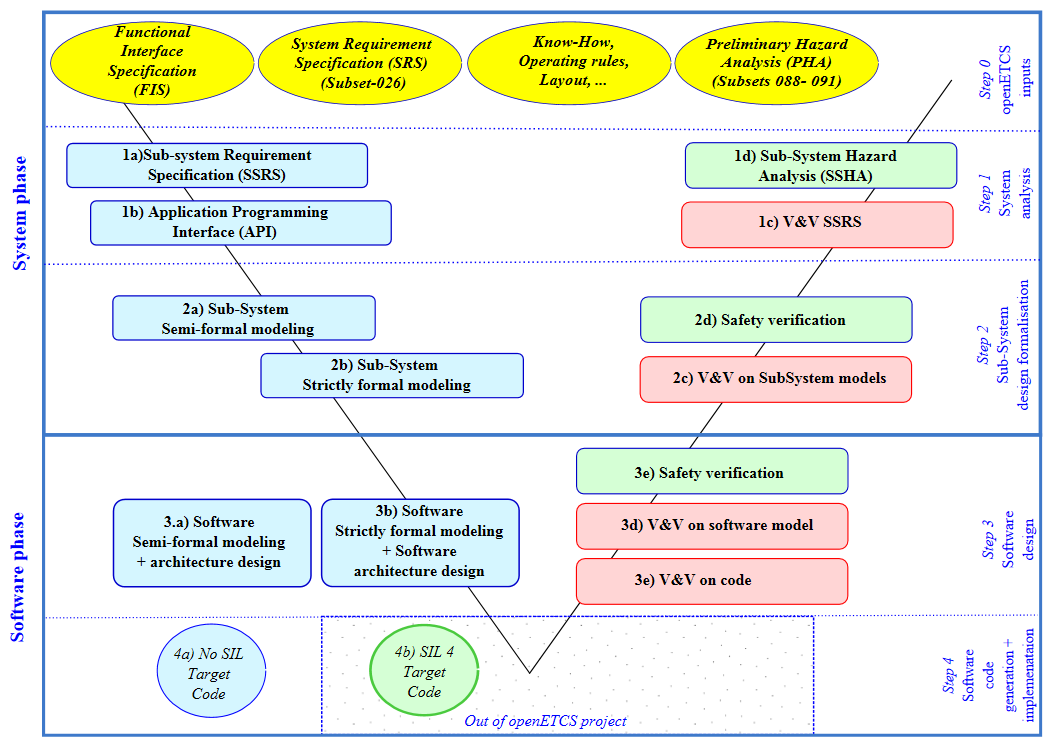
\includegraphics[width=.9\textwidth]{images/ProcessOpenETCS-BeM.png}
  \caption{openETCS Process (rough view)}
  \label{fig:frama-c-openETCSProcess}
\end{figure}

According figure \ref{fig:frama-c-openETCSProcess}, for which activities is the mean or tool suitable (see also \citep{D4.1} section 5.1.2 for more details)\footnote{DAS2V : Design Artifact Subject to Verification and Validation, see \citep{D4.1}} ?


\begin{tabular}{|l | c | c | c | c|}
\hline
& \textcolor{green}{Author} & \textcolor{blue}{Assessor 1} & \textcolor{magenta}{Assessor 2} & Total \\
\hline 
1c SSRS Verification & 0 & & &  \\
\hline
1c SSRS Validation & 0 & & &  \\
\hline
2c SFM Verification & 0 & & &  \\
\hline
2c SFM Validation & 0 & & &  \\
\hline
3d SW-SFM Verification & 0 & & &  \\
\hline
3d SW-SFM Validation & 0 & & &  \\
\hline
3d SW-FFM Verification & 2 & & &  \\
\hline
3d SW-FFM Validation & 2 & & &  \\
\hline
3e Code Verification & 3 & & &  \\
\hline
3e Code Validation & 3 & & &  \\
\hline
DAS2V Verification & 0 & & &  \\
\hline
DAS2V Validation & 0 & & &  \\
\hline
Automatic model transformation verification & 0 & & &  \\
\hline
Automatic code generation verification & 3 & & &  \\
\hline
\end{tabular}


\section{Properties}

Which kind of properties or elements are verified or validated by the mean or tool (see also \citep{D4.1} section 4)  ?



\begin{tabular}{|l | c | c | c | c|}
\hline
& \textcolor{green}{Author} & \textcolor{blue}{Assessor 1} & \textcolor{magenta}{Assessor 2} & Total \\
\hline 
Functionalities of the system and sub-system & 1 & & &  \\
\hline
System and sub-system architecture & 0 & & &  \\
\hline
External and internal interfaces of sub-system & 0 & & &  \\
\hline
Software components & 3 & & &  \\
\hline
Performance constraints & 1 & & &  \\
\hline
Safety objectives & 0 & & &  \\
\hline
Functional properties & 3 & & &  \\
\hline
Safety properties & 0 & & &  \\
\hline
\end{tabular}



\section{Verification methods and tools}

Which kind of methods is proposed (see also \citep{D4.1} section 5.3) ?



\begin{tabular}{|l | c | c | c | c|}
\hline
& \textcolor{green}{Author} & \textcolor{blue}{Assessor 1} & \textcolor{magenta}{Assessor 2} & Total \\
\hline 
Reviews & 0 & & &  \\
\hline
Inspections & 0 & & &  \\
\hline
Software Architecture Analysis Method & 0 & & &  \\
\hline
Architecture Tradeoff Analysis Method & 0 & & &  \\
\hline
Model-Based System Integration Testing & 0 & & &  \\
\hline
Model-Based Testing of Generated High-Level Code & 0 & & &  \\
\hline
Abstract Interpretation & 3 & & &  \\
\hline
Deductive Verification & 3 & & &  \\
\hline
Model Checking & 1 & & &  \\
\hline
Correct by Construction Formal Methods & 0 & & &  \\
\hline
Verification with Formal Methods & 3 & & &  \\
\hline
Simulation-based & 1 & & &  \\
\hline
\end{tabular}
\begin{author_comment}
Value analysis plug-in can be tweaked to perform some 
model-checking and simulation tasks
\end{author_comment}

\section{Validation means and tools}

The following list of criteria focuss on means and tools to support validation activities, according WP2  requirements :

\begin{tabular}{|l | c | c | c | c|}
\hline
& \textcolor{green}{Author} & \textcolor{blue}{Assessor 1} & \textcolor{magenta}{Assessor 2} & Total \\
\hline 
Simulation-based & 1 & & &  \\
\hline
Step-by-step simulation (D2.6-01-036) & 1 & & &  \\
\hline
Environment emulation (D2.6-01-037 and D2.6-02-080) & 1 & & &  \\
\hline
Time-based test case (D2.6-02-081) & 0 & & &  \\
\hline
Test cases writing (D2.6-01-038) & 1 & & &  \\
\hline
Test cases execution (D2.6-01-038) & 1 & & &  \\
\hline
Test cases storage (D2.6-01-038) & 0 & & &  \\
\hline
Version management of test cases (D2.6-02-082) & 0 & & &  \\
\hline
Test generation from independant test model (D2.6-02-083) & 0 & & &  \\
\hline
Test sequences writing (D2.6-02-084) & 0 & & &  \\
\hline
Test sequences execution (D2.6-02-084) & 0 & & &  \\
\hline
Test sequences storage (D2.6-02-084) & 0 & & &  \\
\hline
\end{tabular}

\section{VnV artifacts}


Concerning the artifacts used or produced by the mean or tool, please to detail:

\paragraph{Input}
\begin{itemize}
\item C code under analysis
\item for functional properties: ACSL contracts specifying the properties of
  interest
\item set of parameters for the plugins that are used.
\end{itemize}
    
    
\paragraph{Output}
\begin{itemize}
\item validity status of each ACSL property
\item (hopefully empty) list of all potential run-time errors that might occur
  during an execution.
\end{itemize}
    
\paragraph{Syntax}
\begin{itemize}
\item ISO/IEC JTC1/SC22/WG14. 9899:TC3: Programming Languages---C
\item ACSL: ANSI/ISO C Specification Language. 
  \url{http://frama-c.com/acsl.html}
\item Frama-C manuals available at \url{http://frama-c.com/}
\end{itemize}
    
\paragraph{Semantic}
See above.


\paragraph{Integration}
    How these artifacts can be integrated with the elements of the toolchain (language, mangement,...) ?


\section{Detailled Criterias for VnV}

Please  fill only the section concerning the proposed mean or tool, other section can be skipped (see issue \url{https://github.com/openETCS/toolchain/issues/180} for details and discussions)



\subsection{System Modelling simulation}	

\begin{tabular}{|l | c | c | c | c|}
\hline
& \textcolor{green}{Author} & \textcolor{blue}{Assessor 1} & \textcolor{magenta}{Assessor 2} & Total \\
\hline 
User Scenario Modelling & & & &  \\
\hline
Test Case Modelling & & & &  \\
\hline
Test Sequence Modelling & & & &  \\
\hline
\end{tabular}
	
\subsection{System Model Verification}	


\begin{tabular}{|l | c | c | c | c|}
\hline
& \textcolor{green}{Author} & \textcolor{blue}{Assessor 1} & \textcolor{magenta}{Assessor 2} & Total \\
\hline 
Input/ Output checking & & & &  \\
\hline
System Behavior Simulation (Mathematical) & & & &  \\
\hline
System Behavior Simulation (Animated) & & & &  \\
\hline
\end{tabular}


\subsection{Software Model Verification	}


\begin{tabular}{|l | c | c | c | c|}
\hline
& \textcolor{green}{Author} & \textcolor{blue}{Assessor 1} & \textcolor{magenta}{Assessor 2} & Total \\
\hline 
Static Model Verification & & & &  \\
\hline
Property Proofing & & & &  \\
\hline
Dynamic Testing & & & &  \\
\hline
Automatic Test Generation & & & &  \\
\hline
Input/ Output checking & & & &  \\
\hline
Software Behaviour Simulation (Mathematical) & & & &  \\
\hline
Software Behaviour Simulation (Animated) & & & &  \\
\hline
\end{tabular}


\subsection{Source Code}


\begin{tabular}{|l | c | c | c | c|}
\hline
& \textcolor{green}{Author} & \textcolor{blue}{Assessor 1} & \textcolor{magenta}{Assessor 2} & Total \\
\hline 
Traceability to Model & 1 & & &  \\
\hline
\end{tabular}

\begin{author_comment}
  If ACSL specifications are generated from the model (see
  section~\ref{sec:Frama-C:language}) with proper traceability
  artifacts, it should be possible to trace back each verification
  condition assessed by Frama-C to the original constraint in the
  model.
\end{author_comment}

\subsection{Code Verification	}


\begin{tabular}{|l | c | c | c | c|}
\hline
& \textcolor{green}{Author} & \textcolor{blue}{Assessor 1} & \textcolor{magenta}{Assessor 2} & Total \\
\hline 
Formal Proof & 3 & & &  \\
\hline
Programming by contract & 3 & & &  \\
\hline
Static Analysis & 3 & & &  \\
\hline
Dynamic Analysis & 1 & & &  \\
\hline
Dynamic Testing & * & & &  \\
\hline
Automatic Test Generation & * & & &  \\
\hline
Performance Testing & 1 & & &  \\
\hline
Interface Testing & 1 & & &  \\
\hline
\end{tabular}
\begin{author_comment}
Value analysis' interpreter mode can be used to perform some dynamic analysis.
As mentioned above, there is a test case generator plugin, but it is not
distributed as free software.
\end{author_comment}
	
\subsection{Validation System/Software/Code/ Validation	}


\begin{tabular}{|l | c | c | c | c|}
\hline
& \textcolor{green}{Author} & \textcolor{blue}{Assessor 1} & \textcolor{magenta}{Assessor 2} & Total \\
\hline 
Test Coverage & & & &  \\
\hline
Use Case Validation of Model & & & &  \\
\hline
Functional or Black-box Testing & & & &  \\
\hline
User Scenario Testing & & & &  \\
\hline
Traceability & & & &  \\
\hline
Schedulability Analyzer / UseCase Check all & & & &  \\
\hline
Schedulability Analyzer / UseCase Check single mode & & & &  \\
\hline

\end{tabular}



\section{Other comments}



\begin{comment}
This section is available for the author or the assessors to  complete the description and criteria.
\end{comment}

Slides of Frama-C presentation are available on github
\url{https://github.com/openETCS/model-evaluation/blob/master/Telco_Secondary_slides/c-frama-c-secondary-tools-presentation.pdf}.

Specification and verification activities over the \texttt{bitwalker} code from
Siemens have been conducted by Fraunhofer FOKUS with support from CEA LIST.
The development is available on github: \url{https://github.com/openETCS/validation/tree/master/VnVUserStories/VnVUserStoryFraunhoferFOKUS}